%中間審査概要テンプレート ver. 3.0

\documentclass[uplatex,twocolumn,dvipdfmx]{jsarticle}
\usepackage[top=22mm,bottom=22mm,left=22mm,right=22mm]{geometry}
\setlength{\columnsep}{10mm}
\setlength\textfloatsep{2pt}
\setlength\intextsep{2pt}
\usepackage[T1]{fontenc}
\usepackage{txfonts}
\usepackage[expert,deluxe]{otf}
\usepackage[dvipdfmx,hiresbb]{graphicx}
\usepackage[dvipdfmx]{hyperref}
\usepackage{pxjahyper}
\usepackage{secdot}





%タイトルと学生番号,名前だけ編集すること
\title{\vspace{-5mm}\fontsize{14pt}{0pt}\selectfont OSS開発者のプロジェクトへの貢献度と社交性の相関分析}
\author{\normalsize プロジェクトマネジメントコース 矢吹研究室 1342081 辻岡 大知}
\date{}
\pagestyle{empty}
\begin{document}
\fontsize{10.5pt}{\baselineskip}\selectfont
\maketitle





%以下が本文
\section{背景}

ソフトウェア開発では,GitHubを用いることが多い.GitHubとはコンピュータ上で作成,編集されるファイルの変更履歴を管理するためのバージョン管理システムである.\cite{a}


システムエンジニアはコミュニケーション能力が必要とされる仕事である.私はGitHubに公開されているプロジェクトを調べているうち,活発に活動しているユーザはGoogle+やTwitterで交友関係が広い場合が多いことに気が付いた.そこで私はGitHubを用い,活発に活動するシステムエンジニアはコミュニティが広いのではないかという仮説を立て,その仮説を検証するため本研究を行った.


\section{目的}

ソフトウェア開発で活発に活動しているユーザはコミュニティが広いのではないかという仮説を検証する.

\section{手法}

活発に活動しているシステムエンジニアのユーザ情報を集めるためGHTorrentを使用した.GHTorrentとはGitHubのユーザ情報やプロジェクトの情報など様々なデータが格納されているダンプファイルのことである.

活発に活動しているシステムエンジニアのコミュニティを調べるため,Google+とGitHubにおけるユーザ情報の一つであるcontributionを使用した.contributionとはユーザがどの程度GitHub上で活動しているのかを定量的に知ることのできる値である.

集めたユーザのコミュニティ関係を調べるためGoogle+を使用した.Google+とはGoogleが運営するSNSのことである.

以下のような手順で研究を進めた.

\begin{enumerate}
 \item GHTorrentから2万件のユーザ情報をランダムサンプリングで抽出した.
 \item 1で抽出したユーザのメールアドレスを,GitHubAPIを用いて取得した.
 \item 取得したメールアドレスを用いGoogle+におけるフォロワー数を調べた.
 \item ユーザのcontribution数とGoogle+におけるフォロワー数の相関関係を調べた.
\end{enumerate}

\section{結果}

本研究の結果が図\ref{サンプル図}の散布図である.回帰分析の結果,重相関Rの値が約0.19となったため,GitHubにおけるcontribution数とGoogle+におけるフォロワー数にほとんど相関はないということが分かった.

%図の挿入
\begin{figure}[ht]
\centering
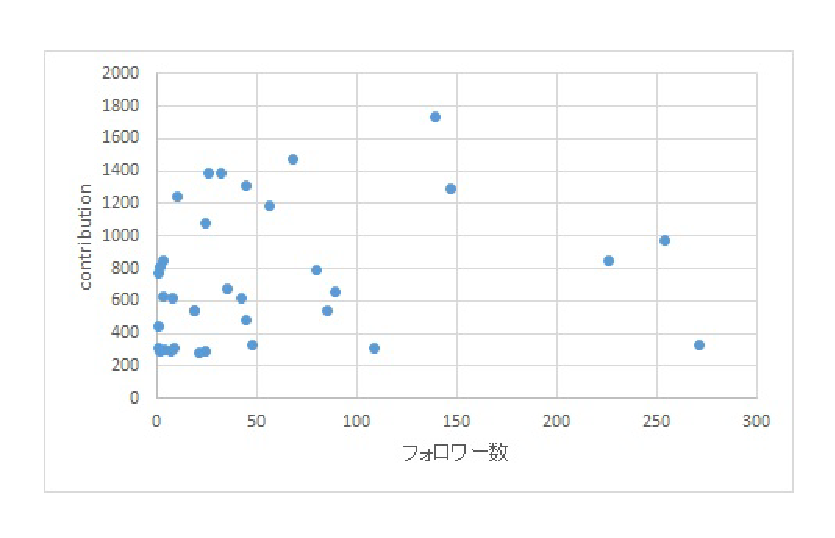
\includegraphics[width=6cm,height=3cm,clip]{figure.pdf}
\caption{contribution数とフォロワー数の相関}
\label{サンプル図}
\end{figure}

\section{考察}

本研究を通して,活発に活動しているユーザはGoogle+におけるコミュニティが必ずしも広いわけではないことが分かった.今回はGoogle+を用いたが,現在流行しているFacebookやTwitterなど他のSNSを用いることにより,今回とは違った結果が得られるのではないかと考えた.

\section{結論}

本研究を通して明らかとなった相関関係などはなかった.しかし研究を進めるための過程でGHTorrent及びGoogleAPIを使用することができるようになった.今後の課題として研究を行う段階で最も流行しているSNSなどでデータを取得し,統計を取っていく必要がある.


\bibliographystyle{junsrt}
\bibliography{biblio}%「biblio.bib」というファイルが必要.



\end{document}
